
\chapter{Présentation de \LaTeX}
\begin{center}
\begin{minipage}[r]{0.5\linewidth}
  Présentation des caractéristiques de la rédaction de documents avec
  \LaTeX. Différences par rapport aux traitements de texte
  WYSIWYG. Sources d'information. Structuration de documents. Notions
  d'instruction et d'environnement.
  \end{minipage}
\end{center}

\include{inputs/presentation-LaTeX}



\chapter{Présentation d'Emacs}
\begin{center}
\begin{minipage}[r]{0.5\linewidth}
  Nous allons apprendre à utiliser l'éditeur de texte Emacs afin de
  pouvoir être plus à l'aise avec la rédaction de documents
  \LaTeX.
  \end{minipage}
\end{center}

\include{inputs/emacs}


\chapter{Premier contact avec \LaTeX}

\begin{center}
\begin{minipage}[r]{0.5\linewidth}
  Ce chapitre a pour but de vous présenter les fondements essentiels
  de la rédaction de textes avec \LaTeX.
  \end{minipage}
\end{center}

\include{inputs/standard-LaTeX}


\chapter{\LaTeX\ et les langues}
\label{cha:babel}
\begin{center}
  \begin{minipage}[r]{0.5\linewidth}
    Prise en charge des spécificités linguistiques avec \LaTeX\
    (typographie, vocabulaire automatique\ldots).
  \end{minipage}
\end{center}



%%%%%%%%%%%%%%%%%%%%%%%%%%%%%%%%%%%%%%%%%%%%%%%%%%%%%%%%%%%%%%%%%%%%%%%%%%%

%%  LaTeX et le français

%%%%%%%%%%%%%%%%%%%%%%%%%%%%%%%%%%%%%%%%%%%%%%%%%%%%%%%%%%%%%%%%%%%%%%%%%%%



\section{\LaTeX\ et les spécificités typographiques}

\begin{itemize}
\item Dans chaque pays, il existe un ensemble de règles typographiques qui ont
  pour objet de réglementer la mise en page des documents écrits.
\item Ces règles sont plus ou moins générales :
  \begin{itemize}
  \item Certaines s'appliquent à tous les supports écrits (le traitement des
    espaces, l'interligne de début de paragraphe, l'indentation de début de
    paragraphe, la césure\ldots).
  \item D'autres sont spécifiques à un type de document (c'est notamment le cas
    des lettres dont la mise en page relève de règles bien particulières en
    fonction des pays).
  \end{itemize}
\end{itemize}


\section{Les espaces et le français}

\begin{itemize}
\item Tout le monde connaît les variations typographiques de base qui sont
  respectivement en usage dans les pays anglophones et francophones.
  \begin{itemize}
  \item Langue anglaise : pas d'espace avant les caractères de ponctuation.
  \item Langue française : espace\footnote{En réalité, les règles
      typographiques françaises imposent un espace d'une taille
      différente de l'espace entre deux mots.} avant les caractères
    \emph{doubles} (\emph{:},\emph{;},\emph{!},\emph{?}) mais pas
    devant les caractères simples.
  \end{itemize}
\item Il est très facile avec \LaTeX\ de gérer ces règles typographiques de
  manière transparente pour l'utilisateur. Sans aller trop loin dans l'étude de
  l'extension \LaTeX\ qui permet de gérer ce problème, nous allons commencer à
  l'utiliser dès maintenant. Ce qui nous permettra d'apprécier la qualité de la
  mise en page quelle que soit la langue utilisée.
\end{itemize}

%\newpage 

Nous allons donc introduire dans l'en-tête du document (avant
\verb1\begin{document}1) l'appel :
  
\begin{flushright}
  \verb1\usepackage[french]{babel}1.
\end{flushright}
  
\begin{exemple}[H]
  \caption{Usage des règles typographiques du français avec \LaTeX}
\begin{verbatim}
\documentclass[a4paper]{article}
\usepackage[utf8]{inputenc}
\usepackage{xspace}
\usepackage[english,french]{babel}

\begin{document}
...
\end{document}
\end{verbatim}
\end{exemple}


Cette extension va notamment avoir pour fonction :

\begin{itemize}
\item D'insérer un espace insécable \emph{avant} les signes de
  ponctuation qui le nécessitent (que vous mettiez vous-même un espace
  ou pas, \emph{babel} se chargera de faire ce qu'il faut pour que la
  taille de l'espace soit toujours la même).
\item D'empêcher les sauts de lignes avant ces espaces (plus de caractères de
  ponctuation en début de ligne) sans que vous ayez quoi que ce soit à faire.
\item De couper (en anglais \emph{hyphenation}, \emph{césure}) les
  mots français où il le faut pour que la mise en page soit agréable.
\item De franciser votre document (la date sera écrite en français notamment).
\item \ldots (nous étudierons l'extension \emph{babel} plus en détails
  par la suite).
\end{itemize}



\section{Francisation automatique du texte}

\begin{itemize}
\item En appelant l'extension \emph{Babel}, les mots qui sont insérés
  automatiquement par \LaTeX\ seront automatiquement francisés :
  \begin{itemize}
  \item bibliography vs. bibliographie
  \item chapter vs. chapitre
  \item Abstract vs. Résumé
  \item Appendix vs. Annexe
  \item Table of contents vs. Table des matières
  \item List of figures vs. Liste des figures
  \item francisation de la date
  \item francisation des titres de figures / tableaux
  \item \ldots
  \end{itemize}
\end{itemize}



\section{Autres paramètres modifiés par l'appel à Babel}

\begin{itemize}
\item modification des \og bullets \fg devant les listes
\item réglage de l'espacement entre les éléments d'une liste
\item permet d'utiliser les instructions \verb1\og1 et \verb1\fg1 respectivement
  pour \og Ouvrir les Guillemets français \fg (og) et \og Fermer les Guillemets
  français \fg (fg).% (ou \verb1<<1 et \verb1>>1).
\item On peut obtenir les guillemets \emph{anglais} avec \verb1``1 et \verb1''1,
  ce qui donne `` et ''. Si vous utilisez Emacs, il convertit automatiquement
  \verb1"1 en guillemets anglais ouvrants ou fermants en fonction de leur
  position par rapport au mot : Si vous tapez \verb1"1 après un espace, il les
  convertit en guillemets ouvrants\ldots sinon en guillemets fermants.
\end{itemize}


\section{Basculer d'une langue à l'autre}

\begin{exemple}[H]
  \caption{Usage des règles typographiques du français avec \LaTeX}
\begin{verbatim}
\documentclass[a4paper]{article}
\usepackage[utf8]{inputenc}
\usepackage{xspace}
\usepackage[english,french]{babel}

\begin{document}
...
\selectlanguage{english}
...
\selectlanguage{french}
...
\selectlanguage{english}
...
\end{document}
\end{verbatim}
\end{exemple}

On utilise aussi l'extension \emph{xspace} qui améliore la gestion des
espaces (par exemple dans le cas des guillemets).

Par défaut, la langue par défaut du document est la dernière langue
déclarée dans l'appel à usepackage.


\section{Rédiger des documents dans d'autres langues}
\label{sec:babel}

Ceci n'est qu'un petit aperçu des possibilités de Babel. Vous pouvez
également rédiger des documents dans bien d'autres langues en
utilisant babel (allemand, espagnol, grec, breton, basque, hébreu,
Hongrois, Russe, Turc\ldots). Pour celà, n'hésitez pas à lire la
documentation de Babel:

\bibentry{babeldoc}.

Comme vous pourrez le remarquer, Babel fonctionne surtout pour des
langues qui s'écrivent de gauche à droite. Pour l'arabe (ainsi que
l'hébreu), on utilise en général l'extension \verb1arabtex1. Pour les
langues comme le chinois, le coréen, le japonais, on utilise
l'extension \verb1CJK1.

N'hésitez pas à chercher sur internet s'il existe une extension qui
soit adaptée à votre langue maternelle ou autre (il existe par exemple
des extensions pour écrire avec les systèmes d'écriture
hiéroglyphique, copte, éthiopien\ldots) et à m'en faire part
(\url{mailto:olivier.crouzet@univ-nantes.fr}) si vous trouvez quelque
chose d'intéressant.

Vous pouvez par exemple consulter la page internet suivante :

\url{http://tug.ctan.org/tex-archive/language/}










\chapter{\LaTeX\ et la linguistique}
\label{cha:babel}
\begin{center}
  \begin{minipage}[r]{0.5\linewidth}
    Quelques liens vers des outils ou des informations utiles pour un
    linguiste utilisant \LaTeX. Transcription phonétique avec
    TIPA. N'hésitez pas à passer rapidement ce chapitre pour y revenir
    plus tard lorsque vous commencerez à maîtriser \LaTeX.
  \end{minipage}
\end{center}

\include{inputs/linguistics-LaTeX}



\chapter{Utilisation avancée de \LaTeX}
\begin{center}
  \begin{minipage}[r]{0.5\linewidth}
    Vous apprendrez à utiliser de nouveaux environnements, de
    nouvelles instructions et à créer des fichiers PDF.
  \end{minipage}
\end{center}

\include{inputs/advanced-LaTeX}


% \chapter{Autres classes de documents \LaTeX}
% \begin{center}
%   \begin{minipage}[r]{0.5\linewidth}
    
%   \end{minipage}
% \end{center}

% \include{inputs/formats-LaTeX}
% report, book
% letter, lettre
% a0poster, beamer 


\chapter{Les objets flottants : insertion de graphiques}
\label{cha:graphiques}
\begin{center}
  \begin{minipage}[r]{0.5\linewidth}
    Vous allez maintenant apprendre à insérer des graphiques ou des
    images et à manipuler ce que l'on appelle des \og objets flottants
    \fg.
  \end{minipage}
\end{center}

\include{inputs/floats-graph-LaTeX}


\chapter{Les objets flottants : insertion de tableaux}
\label{cha:tableaux}
\begin{center}
  \begin{minipage}[r]{0.5\linewidth}
    Les tableaux sont aussi des objets qui peuvent flotter. Nous
    allons donc retrouver certains points abordés dans le cas des
    graphiques. Mais vous allez aussi apprendre à créer des tableaux
    de données. Cette partie devrait vous prendre beaucoup de temps
    car, si les tableaux produits par LaTeX peuvent être d'une qualité
    typographique exceptionnelle, ceci demandera beaucoup de travail
    de votre part.
  \end{minipage}
\end{center}



\section{Les tableaux}
\label{tableaux}

\vfill 

Comme pour les graphiques, deux points indépendants sont à considérer :

\begin{itemize}
\item La création d'un tableau dans un document \LaTeX\ (cf.~\ref{tabular}).
\item Le positionnement du tableau et de son titre dans le document (retour à la
  notion de flottant, cf.~\ref{table}).
\end{itemize}

\vfill







\section{Créer un tableau avec les outils standards}
\label{tabular}

\vfill

\begin{boxedminipage}{\textwidth}
\begin{verbatim}
\begin{tabular}{spécification des colonnes}
donnée & donnée & donnée & ... & donnée \\
donnée & donnée & donnée & ... & donnée \\
...
\end{tabular}
\end{verbatim}
\end{boxedminipage}

\begin{itemize}
\item Instructions utiles
  \begin{itemize}
  \item \verb1\hline1 : trace une ligne horizontale sur toute la largeur du
    tableau;
  \item \verb1\cline{N-M}1 : trace une ligne horizontale des colonnes N à M;
  \item \verb1\multicolumn{nbcols}{format}{Texte étendu sur plusieurs colonnes}1
  \item la déclaration des colonnes se fait avec les lettres \emph{c,
      l, r} (center, left, right). On indique autant de lettres que
    l'on veut de colonnes, chaque lettre indique l'alignement du texte
    dans la colonne;
  \item Les \verb1&1 servent à sépararer les colonnes;
  \item On indique la fin de ligne par \verb1\\1.
  \end{itemize}
\end{itemize}

%%Nous allons voir quelques exemples de l'utilisation de \emph{tabular} :
\vfill

\section{Exercices}

\begin{itemize}
\item Construisez, sur papier, un tableau très simple (3 colonnes, 5
  lignes) et reproduisez le avec \LaTeX\ en traçant toutes les lignes
  verticales et horizontales;
\item Reproduisez ce même tableau en supprimant toutes les lignes;
\item Reproduisez pour finir ce même tableau en n'introduisant que les
  lignes horizontales;
\item Reproduisez ensuite le tableau présenté ci-dessous en utilisant
  les instructions nécessaires.
\end{itemize}

\begin{center}
  \begin{tabular}{|l|cr|l|} \hline
    Alignement à gauche & Données centrées & et à droite & Largeur imposée\\ \cline{2-3}
    Donnée & \multicolumn{2}{|c|}{Donnée} & \\ \hline
    1.10 & 2.20 & 3.20 & 4.69 \\
    1.10 & 2.20 & 3.20 & 4.69 \\
    1.10 & 2.20 & 3.20 & 4.69 \\ \hline
  \end{tabular}
\end{center}


\section{L'environnement \emph{tabular}: réponse à la question
  précédente}

\begin{boxedminipage}{\textwidth}
\footnotesize
\begin{verbatim}
\begin{center}
  \begin{tabular}{|l|cr|l|} \hline
    Alignement à gauche & Données centrées & et à droite & Largeur imposée\\ \cline{2-3}
    Donnée & \multicolumn{2}{|c|}{Donnée} & \\ \hline
    1.10 & 2.20 & 3.20 & 4.69 \\
    1.10 & 2.20 & 3.20 & 4.69 \\
    1.10 & 2.20 & 3.20 & 4.69 \\ \hline
  \end{tabular}
\end{center}
\end{verbatim}
\end{boxedminipage}

\begin{center}
  \begin{tabular}{|l|cr|l|} \hline
    Alignement à gauche & Données centrées & et à droite & Largeur imposée\\ \cline{2-3}
    Donnée & \multicolumn{2}{|c|}{Donnée} & \\ \hline
    1.10 & 2.20 & 3.20 & 4.69 \\
    1.10 & 2.20 & 3.20 & 4.69 \\
    1.10 & 2.20 & 3.20 & 4.69 \\ \hline
  \end{tabular}
\end{center}

%% Problèmes de tabular :

%% - contrôle de la largeur des cellules (array, tabularx)
%% - centrage vertical du texte dans la cellule (array)
%% - écartement entre le texte et les lignes horizontales (booktabs)

%% - tableaux longs à introduire sur plusieurs pages (longtable)

%% - multirow : regroupement vertical de cellules (doit-on vraiment l'aborder ?)


\section{Quelques problèmes centraux dans la composition d'un tableau}

\vfill

\subsection{Largeur des cellules}

Pour les colonnes contenant du texte de longueur importante, il faut
indiquer la largeur de colonne souhaitée, sinon l'on obtient quelque
chose d'assez désagréable : \LaTeX\ attribue à la cellule la largeur
du texte qu'elle contient (ce qui peut être vraiment grand !).

\subsection{Alignement vertical du texte}

L'environnement \emph{tabular} standard ne permet pas de contrôler
l'alignement vertical. Le texte est nécessairement aligné avec le haut
de la cellule.

\subsection{\'Ecartement texte / ligne horizontale}

Certaines lettres (les majuscules) touchent la ligne horizontale qui les domine.

\vfill


\section{Illustrations}

\subsection{Largeur des cellules}

\begin{boxedminipage}{\textwidth}
\begin{verbatim}
\begin{tabular}{|l|cr|c|} \hline
  Donnée & Donnée & Donnée & Ici un texte relativement long...\\ \hline
\end{tabular}
\end{verbatim}
\end{boxedminipage}

\begin{center}
  \begin{tabular}{|l|cr|c|} \hline
    Donnée & Donnée & Donnée & Sinon, \LaTeX\ adapte la taille de la colonne à la taille du texte. Ce qui peut poser des problèmes.\\ \hline
    % Donnée & Donnée & Donnée & \\ \hline
  \end{tabular}
\end{center}

\subsection{Alignement vertical}

\begin{tabular}{|p{.5\textwidth}|ccc|} \hline
  Texte relativement long blah blah blah blah blah blah blah blah blah blah blah blah blah blah blah blah blah blah & A & A & A \tabularnewline \cline{2-4}
  & A & A & A \tabularnewline \cline{2-4}
  & B & B & B \tabularnewline \hline
\end{tabular}


\subsection{Espacement caractère / ligne}

Le problème de l'espacement entre les caractères et la ligne
horizontale est manifeste dans ces deux exemples.



\section{Contrôle de la largeur des colonnes}

\vfill

On dispose de plusieurs solutions dont le choix dépend de la
situation et des préférences de l'utilisateur.


\begin{enumerate}
\item L'utilisateur souhaite laisser \LaTeX\ gérer lui-même la largeur des
  colonnes (gestion automatique) : utiliser l'extension \emph{tabularx}
\item L'utilisateur souhaite avoir le contrôle total de la largeur de chaque
  colonne : utiliser l'extension \emph{array}.
\end{enumerate}

Deux possibilités peuvent apparaître :
\begin{enumerate}
\item \label{toutes}Toutes les cases de la colonne vont contenir un texte de
  ce type. On utilise une technique de définition des colonnes avec l'appel à
  l'extension \emph{array}.
\item \label{titre}Seule une case (souvent dans la ligne de titre ou
  dans la colonne de gauche) contient un texte long, le reste
  contenant des données (par exemple numériques). On pourra utiliser
  soit \emph{array}, soit \emph{tabularx}.
\end{enumerate}

Pour le problème de l'espacement entre lignes horizontales et
caractères, on utilisera l'extension \emph{booktab}.

\vfill




% \section{Première situation}

% \begin{boxedminipage}{\textwidth}
% \begin{verbatim}
% \begin{center}
%   \begin{tabular}{|l|cr|p{.3\textwidth}|} \hline
%     Donnée & Donnée & Donnée & \begin{center}Et une case...\end{center}\\ \hline
%     ...
%     Donnée & \multicolumn{2}{|c|}{Donnée} & \\ \hline
%   \end{tabular}
% \end{center}
% \end{verbatim}
% \end{boxedminipage}


% \begin{center}
%   \begin{tabular}{|l|cr|p{.3\textwidth}|} \hline
%     Donnée & Donnée & Donnée & \begin{center}Et une case du tableau qui contient beaucoup de texte. La dimension de cette case est fixée, pas automatique.\end{center}\\ \hline
%     Donnée & Donnée & Donnée & \begin{center}Et une case du tableau qui contient beaucoup de texte. La dimension de cette case est fixée, pas automatique.\end{center}\\ \hline
%     Donnée & \multicolumn{2}{|c|}{Donnée} & \\ \hline
%   \end{tabular}
% \end{center}







% \section{Seconde situation}

%  \begin{boxedminipage}{\textwidth}
%  \begin{verbatim}
%  \begin{center}
%  \begin{tabular}{|l|cr|r|} \hline
%  Don. & Don. & Don. & \begin{minipage}{.4\textwidth} TEXTE \end{minipage}\\ \hline
%  1.10 & 2.20 & 3.20 & 4.69 \\
%  1.10 & 2.20 & 3.20 & 4.69 \\
%  1.10 & 2.20 & 3.20 & 4.69 \\ \hline
%  \end{tabular}
%  \end{center}
%  \end{verbatim}
%  \end{boxedminipage}

%  \begin{center}
%  \begin{tabular}{|l|cr|r|} \hline
%  Donnée & Donnée & Donnée & \begin{minipage}{.4\textwidth}Et une case du tableau qui contient beaucoup de texte. La dimension de cette case est fixée, pas automatique.\end{minipage}\\ \hline
%  1.10 & 2.20 & 3.20 & 4.69 \\
%  1.10 & 2.20 & 3.20 & 4.69 \\
%  1.10 & 2.20 & 3.20 & 4.69 \\ \hline
%  \end{tabular}
%  \end{center}

%  Quelques problèmes persistent :

%  \begin{itemize}
%  \item Comment joindre deux cellules verticalement ? (multirow)
%  \item Comment centrer le texte verticalement dans les cases ? (array)
%    \begin{itemize}
%    \item Remarquez qu'en utilisant minipage au lieu de \verb1p{largeur}1, les
%      autres cellules sont centrées verticalement.
%    \end{itemize}
%  \item Le texte des données chevauche les lignes horizontales du tableau
%    (booktab)
%  \end{itemize}







\section{L'extension \emph{tabularx}}

\vfill

\begin{itemize}
  
\item On appelle l'extension \emph{tabularx} et on utilise
  l'environnement \emph{tabularx}.

\begin{boxedminipage}{\textwidth}
\begin{verbatim}
\usepackage{tabularx}
...
\begin{tabularx}{.9\textwidth}{Xccc}
...
\end{tabularx}
\end{verbatim}
\end{boxedminipage}


\item On indique la largeur souhaitée pour tout le tableau (par
  exemple 90\% de la largeur de la page) et on marque les colonnes à
  faire varier automatiquement par un X. Les autres colonnes prennent
  la largeur du texte qu'elles contiennent (fonctionnement classique
  de \LaTeX).

\begin{tabularx}{.9\textwidth}{|X|ccc|} \hline
Texte relativement long blah blah blah blah blah blah blah blah blah blah blah blah blah blah blah blah blah blah & A & A & A \tabularnewline \cline{2-4}
& A & A & A \tabularnewline \cline{2-4}
& B & B & B \tabularnewline \hline
\end{tabularx}

\item Problèmes de tabularx : ne permet pas de contrôler l'alignement
  vertical du texte dans les cellules (toujours aligné en
  haut). L'apparence finale est --de mon point de vue-- nettement
  moins agréable qu'avec le contrôle fourni par \emph{array}.

\end{itemize}

\vfill




\section{L'extension \emph{array}}

\begin{itemize}
\item On appelle l'extension \emph{array} dans l'en-tête du document par
  \verb1\usepackage{array}1.
\item L'utilisation est ensuite exactement la même que dans la version standard
  de \LaTeX. (environnement tabular).
\item Par exemple :

  \begin{boxedminipage}{\textwidth}
\small
\begin{verbatim}
\begin{tabular}{b{.5\textwidth}b{.1\textwidth}cc} \hline
Texte relativement long blah ... & A & A & A \\ \cline{2-4}
                            & A & A & A \\ \cline{2-4}
                            & B & B & B \\ \hline
\end{tabular}
\end{verbatim}
  \end{boxedminipage}

\item donne :

\begin{tabular}{b{.5\textwidth}b{.1\textwidth}cc} \hline
Texte relativement long blah blah blah blah blah blah blah blah blah blah blah blah blah blah blah blah blah blah & A & A & A \tabularnewline \cline{2-4}
& A & A & A \\ \cline{2-4}
& B & B & B \\ \hline
\end{tabular}

\item Chaque colonne se voit attribuer une largeur fixée par le
  rédacteur. Le texte qui est plus large que cette colonne est
  \emph{plié} aux dimensions de la colonne. Vous remarquez que les
  déclarations des colonnes sont, pour certaines, très différentes :
  on a remplacé une lettre (c, l ou r) par la commande
  \verb1b{.5\textwidth}1 par exemple pour la première colonne. Les
  colonnes déclarées c, l ou r continuent d'être gérées classiquement
  (largeur automatique attribuée par \LaTeX).

\end{itemize}

\section{Améliorer l'usage de l'extension \emph{array}}

\begin{itemize}
\item \emph{array} fournit la possibilité de définir \emph{au préalable} des
  déclarations pour les colonnes.
\item L'instruction \verb1\newcolumntype{lettre}{définition}1 permet, avant la
  composition du tableau, de définir les caractéristiques des colonnes en leur
  attribuant des types.
\item Exemple :
\begin{verbatim}
\newcolumntype{t}{b{.40\textwidth}}
\newcolumntype{d}{b{.10\textwidth}}
\end{verbatim}
\item Définit 2 nouveaux types de colonnes : t (40\% de la largeur du
  texte, texte aligné sur le bas de la cellule) et d (10\% de la
  largeur du texte et texte également aligné sur le bas de la
  cellule).
\item On peut alors utiliser les lettres \emph{t} et \emph{d} à la place (ou en
  alternance) des lettres \emph{l}, \emph{c} ou \emph{r}.
\item Cette fonctionnalité permet même de modifier d'autres caractéristiques des
  cellules : notamment la police utilisée, la taille\ldots
\begin{verbatim}
\newcolumntype{t}{>{\slshape}b{.40\textwidth}}
\newcolumntype{d}{>{\centering\ttfamily\small}b{.10\textwidth}}
\end{verbatim}
\item Attention cependant : remplacer \verb1\\1 par \verb1\tabularnewline1 pour
  marquer les fins de lignes du tableau.
\end{itemize}




\section{Règle d'utilisation de \emph{newcolumntype}}

\begin{center}
\begin{verbatim}
    \newcolumntype{t}{>{formatage}b{.40\textwidth}}
\end{verbatim}
\end{center}

\begin{itemize}
\item Où le formatage peut servir à déclarer un choix de type de police :
  \begin{itemize}
  \item \verb1\rmfamily1 : Roman (= Serif, cf. Times)
  \item \verb1\sffamily1 : Sans Serif (cf. Helvetica)
  \item \verb1\ttfamily1 : Typewriter (cf. Courier) \emph{Particulièrement utile
      pour les colonnes de chiffres}
  \end{itemize}
\item une orientation des caractères :
  \begin{itemize}
  \item \verb1\slshape1 : Slanted (italique)
  \item \verb1\upshape1 : Droit (par défaut)
  \item \verb1\scshape1 : Small Caps (petites capitales)
  \end{itemize}
\item une graisse :
  \begin{itemize}
  \item \verb1\bfseries1 : Gras
  \end{itemize}
\item un alignement horizontal :
  \begin{itemize}
  \item \verb1\centering1 : Centré
  \item \verb1\raggedleft1 : Repoussé depuis la gauche (Aligné à droite)
  \item \verb1\raggedright1 : Repoussé depuis la droite (Aligné à gauche)
  \end{itemize}
\item une taille de caractères :
  \begin{itemize}
  \item \verb1\tiny1 : du plus petit
  \item \verb1\scriptsize1 : \ldots
  \item \verb1\footnotesize1 : \ldots
  \item \verb1\small1 : \ldots
  \item \verb1\normalsize1 : \ldots
  \item \verb1\large1 : \ldots
  \item \verb1\Large1 : \ldots
  \item \verb1\LARGE1 : \ldots
  \item \verb1\huge1 : \ldots
  \item \verb1\Huge1 : au plus grand
  \end{itemize}
\end{itemize}

Exemple : \verb2\newcolumntype{d}{>{\ttfamily\raggedleft}b{.1\textwidth}}2

Ces déclarations sont des commandes standard de \LaTeX\ (on peut les
utiliser ailleurs pour changer les caractéristiques d'un texte par
exemple).

\section{Un exemple plus complet : alignement sur le bas de la cellule}

\begin{boxedminipage}{\textwidth}
\begin{verbatim}
\newcolumntype{t}{>{\slshape\centering}b{.40\textwidth}}
\newcolumntype{d}{>{\ttfamily\raggedleft}p{.10\textwidth}}

\begin{center}
\begin{tabular}{tddd} \hline
Texte relativement long blah... & A & A & A \tabularnewline \cline{2-4}
        & A & A & A \tabularnewline \cline{2-4}
        & B & B & B \tabularnewline \hline
\end{tabular}
\end{center}
\end{verbatim}
\end{boxedminipage}

\newcolumntype{t}{>{\slshape\centering}b{.40\textwidth}}
\newcolumntype{d}{>{\ttfamily\raggedleft}p{.10\textwidth}}

\begin{center}
\begin{tabular}{tddd} \hline
Texte relativement long blah blah blah blah blah blah blah blah blah blah blah blah blah blah blah blah blah blah & A & A & A \tabularnewline \cline{2-4}
& A & A & A \tabularnewline \cline{2-4}
& B & B & B \tabularnewline \hline
\end{tabular}
\end{center}



\section{Un exemple plus complet : alignement sur le milieu vertical
  de la cellule}

\begin{boxedminipage}{\textwidth}
\begin{verbatim}
\newcolumntype{t}{>{\slshape\centering}m{.40\textwidth}}
\newcolumntype{d}{>{\ttfamily\raggedleft}p{.10\textwidth}}

\begin{center}
\begin{tabular}{tddd} \hline
Texte relativement long blah... & A & A & A \tabularnewline \cline{2-4}
        & A & A & A \tabularnewline \cline{2-4}
        & B & B & B \tabularnewline \hline
\end{tabular}
\end{center}
\end{verbatim}
\end{boxedminipage}

\newcolumntype{t}{>{\slshape\centering}m{.40\textwidth}}
\newcolumntype{d}{>{\ttfamily\raggedleft}p{.10\textwidth}}

\begin{center}
\begin{tabular}{tddd} \hline
Texte relativement long blah blah blah blah blah blah blah blah blah blah blah blah blah blah blah blah blah blah & A & A & A \tabularnewline \cline{2-4}
& A & A & A \tabularnewline \cline{2-4}
& B & B & B \tabularnewline \hline
\end{tabular}
\end{center}







\section{Notes sur l'utilisation de l'extension \emph{array}}

\vfill{}

\begin{itemize}
\item Attention : la largeur de la colonne est en réalité la largeur du texte
  contenu dans la colonne (non compris les espaces gauche et droit autour du
  texte). On risque donc de dépasser la largeur du texte si la somme des
  largeurs de colonnes est égale à 100\% (il suffit de le savoir).
\item L'usage de l'instruction \verb2b{.1\textwidth}2 indique que la colonne
  doit avoir une largeur équivalente à 10\% de la largeur totale du texte sur la
  page \emph{et} que ce texte doit être aligné sur la bas de la cellule (b =
  bottom). On peut aussi centrer le texte verticalement (remplacer \emph{b} par
  \emph{m}).  \emph{p} produit le fonctionnement standard (alignement sur le
  haut de la cellule).
\item La déclaration du type d'alignement vertical est attribuée à une
  colonne mais, évidemment, son effet va porter sur les lignes ! Il
  faut le comprendre comme une indication du type d'alignement qu'on
  va obtenir du texte contenu dans les autres colonnes par rapport à
  la cellule correspondante : si une cellule de la colonne 1 (type
  \verb1t1) contient beaucoup de texte, les autres cellules de la même
  ligne seront alignées sur le bas de cette première cellule. Dans les
  exemples précédents, si une cellule des 3 colonnes de gauche
  contenait beaucoup de texte, le texte des autres cellules serait
  aligné sur le haut de cette cellule !
 \item Noter qu'il est tout à fait possible d'alterner, dans un même document,
   l'usage des environnements \emph{tabular} et \emph{tabularx} en fonction des
   besoins.
\end{itemize}

\vfill{}



%% \section{L'extension \emph{multirow}}

%% \vfill

%% Utilisation de l'extension :

%% \begin{boxedminipage}{\textwidth}
%% \begin{verbatim}
%% \usepackage{multirow}

%% \begin{tabular}{lr} \hline
%% \multirow{nbrows}{largeur}[décalage]{Texte} & donnée \\
%%                                     & donnée \\ \hline
%% \end{tabular}
%% \end{verbatim}
%% \end{boxedminipage}

%% Nous verrons quel peut être l'usage de l'option [décalage] tout à l'heure. Pour
%% l'instant, nous souhaitons essentiellement voir comment écrire du texte dans
%% deux cellules (comment regrouper des cellules).

%% \vfill

%% \section{Utilisation de \emph{multirow}}


%% \begin{boxedminipage}{\textwidth}
%% \begin{verbatim}
%% \begin{center}
%% \begin{tabular}{|c|cp{.3\textwidth}|} \hline
%% \multirow{2}{*}{Titre commun} & Donnée & Un texte relativement ... \\ \cline{2-3}
%%                         & Donnée & Donnée \\ \hline
%% \multirow{2}{.2\textwidth}{Titre long} & Donnée & Un texte ... \\ \cline{2-3}
%%                         & Donnée & Donnée \\ \hline
%% \end{tabular}
%% \end{center}
%% \end{verbatim}
%% \end{boxedminipage}



%% \begin{center}
%% \begin{tabular}{|c|cp{.3\textwidth}|} \hline
%% \multirow{2}{*}{Titre commun} & Donnée & Un texte relativement long pour voir l'effet des cellules qui contiennent beaucoup de texte sur la mise en page du tableau. \\ \cline{2-3}
%%                         & Donnée & Donnée \\ \hline
%% \multirow{2}{.2\textwidth}{Titre commun qui contient plus de texte que n'en pourrait contenir une seule cellule, vraiment beacoup plus} & Donnée & Un texte relativement long pour voir l'effet des cellules qui contiennent beaucoup de texte sur la mise en page du tableau. \\ \cline{2-3}
%%                         & Donnée & Donnée \\ \hline
%% \end{tabular}
%% \end{center}

%% %% \begin{center}
%% %% \begin{tabular}{|c|cc|} \hline
%% %% \multirow{2}{*}{Titre commun} & Donnée & \begin{minipage}{.3\textwidth}Un texte relativement long pour voir l'effet des cellules qui contiennent beaucoup de texte sur la mise en page du tableau.\end{minipage} \\ \cline{2-3}
%% %%                         & Donnée & Donnée \\ \hline
%% %% \multirow{2}{.2\textwidth}{Titre commun qui contient plus de texte que n'en pourrait contenir une seule cellule} & Donnée & \begin{minipage}{.3\textwidth}Un texte relativement long pour voir l'effet des cellules qui contiennent beaucoup de texte sur la mise en page du tableau.\end{minipage} \\ \cline{2-3}
%% %%                         & Donnée & Donnée \\ \hline
%% %% \end{tabular}
%% %% \end{center}


%% Elle permet d'améliorer la mise en page du tableau, notamment lorsque celui-ci
%% contient des cellules qui doivent inclure une grande quantité de texte. Elle
%% utilise la même syntaxe que \emph{tabular}.

%% On l'appelle dans l'en-tête du document par \verb1\usepackage{array}1 et on
%% définit la largeur des cellules pour lesquelles on ne souhaite pas de contrôle
%% automatique en utilisant \verb1m{largeur}1 au lieu de \verb1p{largeur}1.

%% Pour faire intervenir \emph{array}, on définit la largeur d'au-moins une
%% cellule.


%% Avec \emph{array} (\verb1\begin{tabular}{|l|cr|m{.3\textwidth}|} \hline1) :
  
%%   \begin{boxedminipage}{\textwidth}
%% \begin{verbatim}
%% \begin{tabular}{|l|cr|m{.3\textwidth}|} \hline
%% Donnée & Donnée & Donnée & \begin{center}Et une case...\end{center}\\ \cline{2-3}
%% Donnée & Donnée & Donnée & \\ \hline
%% \end{tabular}
%% \end{verbatim}
%%   \end{boxedminipage}

%% \begin{center}
%% \begin{tabular}{|l|cr|m{.3\textwidth}|} \hline
%% Donnée & Donnée & Donnée & \begin{center}Et une case du tableau qui contient beaucoup de texte. La dimension de cette case est fixée, pas automatique.\end{center}\\ \cline{2-3}
%% Donnée & Donnée & Donnée & \\ \hline
%% \end{tabular}
%% \end{center}

%% \newpage

%% et sans \emph{array} (\verb1\begin{tabular}{|l|cr|p{.3\textwidth}|} \hline1) :

%%   \begin{boxedminipage}{\textwidth}
%% \begin{verbatim}
%% \begin{tabular}{|l|cr|p{.3\textwidth}|} \hline
%% Donnée & Donnée & Donnée & \begin{center}Et une case...\end{center}\\ \cline{2-3}
%% Donnée & Donnée & Donnée & \\ \hline
%% \end{tabular}
%% \end{verbatim}
%%   \end{boxedminipage}

%% \begin{center}
%% \begin{tabular}{|l|cr|p{.3\textwidth}|} \hline
%% Donnée & Donnée & Donnée & \begin{center}Et une case du tableau qui contient beaucoup de texte. La dimension de cette case est fixée, pas automatique.\end{center}\\ \cline{2-3}
%% Donnée & Donnée & Donnée & \\ \hline
%% \end{tabular}
%% \end{center}


\section{Le problème du chevauchement lettres / lignes}

Vous avez probablement remarqué que les lignes horizontales des tableaux
chevauchent le haut de certaines lettres.


\begin{itemize}
\item Pour empêcher les lettres de chevaucher les lignes horizontales du
  tableau, on peut introduire une instruction (à n'importe quel endroit du
  document mais en général dans l'en-tête):
  \begin{itemize}
  \item \verb1\setlength{\extrarowheight}{dimension}1
  \end{itemize}
\item Dans le tableau précédent, les lettres hautes (notamment les majuscules)
  touchent les lignes horizontales qui les dominent.
\item Si on ajoute \verb1\setlength{\extrarowheight}{0.3em}1, dans l'en-tête du
  document ou avant de composer le tableau, on obtient :
  \setlength{\extrarowheight}{0.3em}

\begin{center}
\begin{tabular}{|t|ddd|} \hline
Texte relativement long blah blah blah blah blah blah blah blah blah blah blah blah blah blah blah blah blah blah & A & A & A \tabularnewline \cline{2-4}
& A & A & A \tabularnewline \cline{2-4}
& B & B & B \tabularnewline \hline
\end{tabular}
\end{center}

% \item Mais cette procédure peut (lorsqu'on utilise des lignes
%   verticales, mais cf p.\ref{regles-table}) produire des vides.
\end{itemize}

Mais l'outil le plus intéressant pour construire les tableaux (en
combinaison avec \emph{array}) est l'extension \emph{booktabs},
développée pour construire des tableaux de qualité pour la publication
de documents écrits.


\section{L'extension \emph{booktabs}}
\label{booktab}
\setlength{\extrarowheight}{0ex}

\vfill
\begin{itemize}
\item \verb1\usepackage{booktabs}1
\item L'extension \emph{booktabs} s'occupe de formater un tableau en respectant
  scrupuleusement les nécessités typographiques en vigueur dans l'édition.
  \begin{itemize}
  \item Amélioration de la gestion des espaces entre les lignes (pas besoin de
    modifier arbitrairement l'espacement entre les lignes et le texte).
  \item Possibilité de faire varier l'épaisseur des lignes (épaisse en haut et
    en bas, fine à l'intérieur du tableau).
  \item Compatible avec \emph{array} (on peut fixer la largeur des colonnes et
    leur alignement vertical par exemple).
  \item Fonctionne aussi avec \emph{longtable} (cf. p.\ref{longtable}).
%  \item Permet d'insérer des sauts de lignes dans un texte relativement long.
  \end{itemize}
\item Notez qu'un tableau de données NE DOIT PAS comporter de lignes
  verticales.
\end{itemize}
\vfill
\newpage

\section{Différences entre \emph{array} et \emph{booktabs}}

\begin{itemize}
\item \emph{array} et \emph{booktabs} peuvent être utilisés simultanément.
\item Mais \emph{booktabs} doit être considéré comme une couche supplémentaire
  qui améliore la mise en page.
  
  \begin{center}
    \begin{tabular}{l!{$\rightarrow$}l} \toprule
      \emph{array} & \emph{booktabs} \tabularnewline \midrule
      \verb1\hline1 & \verb1\toprule1 \tabularnewline
      & \verb1\midrule1 \tabularnewline
      & \verb1\bottomrule1 \tabularnewline \midrule
      \verb1\cline{N-M}1 & \verb1\cmidrule{N-M}1 \tabularnewline \bottomrule
    \end{tabular}
  \end{center}
\end{itemize}

Notez que les épaisseurs de lignes peuvent ne pas apparaître
correctement à l'écran (visualisation PDF) mais apparaîtront
correctement à l'impression.


\section{Exemple d'utilisation de \emph{booktabs}}

\begin{boxedminipage}{\textwidth}
\begin{verbatim}
\usepackage{booktabs}

\begin{tabular}{lcrrr} \toprule
  & & Condition 1 & Condition 2 & Condition 3 \tabularnewline \midrule
  Expérience 1 & Temps de réaction (en ms) & 600 & 700 & 800 \tabularnewline
  & Taux d'erreur (en \%)  & 14 & 10 & 4 \tabularnewline \cmidrule{2-5}
  Expérience 2 & Temps de réaction (en ms) & 700 & 700 & 700 \tabularnewline
  & Taux d'erreur (en \%)  & 14 & 24 & 34 \tabularnewline \midrule
\end{tabular}
\end{verbatim}
\end{boxedminipage}

\begin{center}
  \begin{tabular}{lcrrr} \toprule
    & & Condition 1 & Condition 2 & Condition 3 \tabularnewline \midrule
    Expérience 1 & Temps de réaction (en ms) & 600 & 700 & 800 \tabularnewline
    & Taux d'erreur (en \%)  & 14 & 10 & 4 \tabularnewline \cmidrule{2-5}
    Expérience 2 & Temps de réaction (en ms) & 700 & 700 & 700 \tabularnewline
    & Taux d'erreur (en \%)  & 14 & 24 & 34 \tabularnewline \midrule
%%     Et même si l'on a \emph{vraiment} besoin d'insérer un texte relativement long dans cette cellule, son formatage est correct & Temps de réaction (en ms) & 700 & 700 & 700 \tabularnewline
%%     & Taux d'erreur (en \%)  & 14 & 24 & 34 \tabularnewline \bottomrule
%%     \multicolumn{3}{l}{\begin{minipage}{.6\textwidth}D'ailleurs un formatage avec extension de la cellule sur la ligne serait certainement plus agréable à lire. Même si le texte qu'elle contient est extrêmement long.\end{minipage}} & &  \\
%%     & Temps de réaction (en ms) & 700 & 700 & 700 \\
%%     & Taux d'erreur (en \%)  & 14 & 24 & 34 \\ \bottomrule
  \end{tabular}
\end{center}


\section{Et en collaboration avec \emph{array}\ldots}

\newcolumntype{t}{>{\slshape\raggedright}b{.20\textwidth}}
\newcolumntype{s}{>{\sffamily}c}
\newcolumntype{d}{>{\ttfamily}r}

\begin{boxedminipage}{\textwidth}
\begin{verbatim}
\newcolumntype{t}{>{\slshape\raggedright}b{.20\textwidth}}
\newcolumntype{s}{>{\sffamily}c}
\newcolumntype{d}{>{\ttfamily}r}

\begin{tabular}{lcrrr} \toprule
  & & Condition 1 & Condition 2 & Condition 3 \tabularnewline \midrule
  Expérience 1 & Temps de réaction (en ms) & 600 & 700 & 800 \tabularnewline
  & Taux d'erreur (en \%)  & 14 & 10 & 4 \tabularnewline \cmidrule{2-5}
  Expérience 2 & Temps de réaction (en ms) & 700 & 700 & 700 \tabularnewline
  & Taux d'erreur (en \%)  & 14 & 24 & 34 \tabularnewline \midrule
\end{tabular}
\end{verbatim}
\end{boxedminipage}

\begin{center}
  \begin{tabular}{tsddd} \toprule
    & & Condition 1 & Condition 2 & Condition 3 \tabularnewline \midrule
    Expérience 1 & Temps de réaction (en ms) & 600 & 700 & 800 \tabularnewline
    & Taux d'erreur (en \%)  & 14 & 10 & 4 \tabularnewline \cmidrule{2-5}
    Expérience 2 & Temps de réaction (en ms) & 700 & 700 & 700 \tabularnewline
    & Taux d'erreur (en \%)  & 14 & 24 & 34 \tabularnewline \midrule
%%     Et même si l'on a \emph{vraiment} besoin d'insérer un texte relativement long dans cette cellule, son formatage est correct & Temps de réaction (en ms) & 700 & 700 & 700 \tabularnewline
%%     & Taux d'erreur (en \%)  & 14 & 24 & 34 \tabularnewline \bottomrule
%%     \multicolumn{3}{l}{\begin{minipage}{.6\textwidth}D'ailleurs un formatage avec extension de la cellule sur la ligne serait certainement plus agréable à lire. Même si le texte qu'elle contient est extrêmement long.\end{minipage}} & &  \\
%%     & Temps de réaction (en ms) & 700 & 700 & 700 \\
%%     & Taux d'erreur (en \%)  & 14 & 24 & 34 \\ \bottomrule
  \end{tabular}
\end{center}


% \section{\ldots et avec \emph{tabularx}}

% \begin{boxedminipage}{\textwidth}
% \begin{verbatim}
% \newcolumntype{s}{>{\slshape\centering}m{.2\textwidth}}

% \begin{tabular}{Xsrrr} \toprule
%   & & Condition 1 & Condition 2 & Condition 3 \tabularnewline \midrule
%   Expérience 1 & Temps de réaction (en ms) & 600 & 700 & 800 \tabularnewline
%   & Taux d'erreur (en \%)  & 14 & 10 & 4 \tabularnewline \cmidrule{2-5}
%   Expérience 2 & Temps de réaction (en ms) & 700 & 700 & 700 \tabularnewline
%   & Taux d'erreur (en \%)  & 14 & 24 & 34 \tabularnewline \midrule
% \end{tabular}
% \end{verbatim}
% \end{boxedminipage}

% %\newcolumntype{s}{>{\slshape}c}
% \newcolumntype{s}{>{\slshape\centering}m{.3\textwidth}}
% \begin{center}
%   \begin{tabularx}{.9\textwidth}{Xsrrr} \toprule
%     & & Condition 1 & Condition 2 & Condition 3 \\ \midrule
%     Expérience 1 & Temps de réaction (en ms) & 600 & 700 & 800 \\
%     & Taux d'erreur (en \%)  & 14 & 10 & 4 \\ \cmidrule{2-5}
%     Expérience 2 & Temps de réaction (en ms) & 700 & 700 & 700 \\
%     & Taux d'erreur (en \%)  & 14 & 24 & 34 \\ \midrule
%   \end{tabularx}
% \end{center}


\section{Rappels essentiels sur la composition d'un tableau de données}
\label{regles-table}
\vfill

La construction d'un tableau répond à des règles strictes qu'il convient de
suivre pour les publications de travaux de recherche. En voici quelques unes
comme bref rappel :

\begin{itemize}
\item Un tableau ne doit jamais contenir de lignes verticales !
  \emph{Jamais} !
\item Les lignes horizontales doivent servir à séparer des éléments
  qui sont extrêments différents les uns des autres. Inutile de
  séparer toutes les lignes du tableau par une ligne horizontale si
  certaines lignes peuvent être groupées ensemble.
\item De fait, deux lignes correspondant à des données qui partagent
  un même en-tête doivent obéir à une règle simple : elles ne sont
  séparées par aucune ligne. Il est inutile --voire gênant-- de
  regrouper des cellules verticalement ; le simple fait que leur
  en-tête soit unique permet d'identifier les lignes comme relevant
  d'une même catégorie.
\item Par ailleurs, il est toujours essentiel, lorsque l'on rencontre
  des problèmes de mise en page, de se poser la question de la
  légitimité typographique de ce que l'on souhaite faire dans un
  tableau.
\item Si vous n'y arrivez pas avec \LaTeX, c'est (peut-être)
  simplement parce que vous devriez changer votre choix\ldots
\item Un tableau doit être le plus succinct possible :
  \begin{itemize}
  \item limiter les textes longs au strict minimum, ceux-ci trouvant plutôt leur
    place dans le corps du texte ou dans le titre du tableau.
  \item Ne pas abuser des changements de police de caractères
    (homogénéité au moins à l'intérieur des colonnes, à part
    éventuellement pour la ligne d'en-tête et la distinction texte /
    nombres).
  \end{itemize}
\item Si vous respectez ces quelques règles, vous ne devriez pas perdre de temps
  dans la composition de vos tableaux.
\end{itemize}

\vfill


% \newpage

% \vfill

% \begin{center}
%   Bon courage !
% \end{center}

% \vfill

%% \section{Un tableau typographiquement correct est en réalité extrêmement simple}

%% \begin{boxedminipage}{\textwidth}
%% \begin{verbatim}
%%   \begin{tabular}{m{.2\textwidth}lrrr} \hline
%%     & & Condition 1 & Condition 2 & Condition 3 \\ \hline
%%     Expérience 1 & Temps de réaction (en ms) & 600 & 700 & 800 \\
%%     & Taux d'erreur (en \%)  & 14 & 10 & 4 \\ \hline
%%     Expérience 2 & Temps de réaction (en ms) & 700 & 700 & 700 \\
%%     & Taux d'erreur (en \%)  & 14 & 24 & 34 \\ \hline
%%     Texte long & Temps de réaction (en ms) & 700 & 700 & 700 \\
%%     & Taux d'erreur (en \%)  & 14 & 24 & 34 \\ \hline
%%   \end{tabular}
%% \end{verbatim}
%% \end{boxedminipage}

%% \begin{center}
%%   \begin{tabular}{m{.2






\newcolumntype{t}{>{\slshape\raggedright}b{.20\textwidth}}
\newcolumntype{s}{>{\sffamily}c}
\newcolumntype{s}{>{\sffamily\centering}b{.20\textwidth}}


\section{Positionnement et attribution d'un titre}
\label{table}

\begin{itemize}
\item Les tableaux sont aussi des objets qui peuvent (et doivent dans
  un texte universitaire, scientifique\ldots) flotter dans le
  document, c'est à dire être placés au meilleur endroit possible et
  être désignés dans le texte par leur numéro.
\item Il faut donc les inclure dans un environnement qui les fera flotter et
  permettra de leur attribuer un titre et, évidemment, une numérotation
  automatique.
\item On procèdera d'une manière similaire à celle que l'on a utilisée pour les
  graphiques, seule la position du titre changera puisque -contrairement aux
  graphiques- les titres de tableaux doivent apparaître au-dessus.
\end{itemize}

\begin{boxedminipage}{\textwidth}
\begin{verbatim}
\begin{table}
\caption{}
\begin{center}
  \begin{tabular}{tsddd} \toprule
    & & Condition 1 & Condition 2 & Condition 3 \tabularnewline \midrule
    Expérience 1 & Temps de réaction (en ms) & 600 & 700 & 800 \tabularnewline
    & Taux d'erreur (en \%)  & 14 & 10 & 4 \tabularnewline \cmidrule{2-5}
    Expérience 2 & Temps de réaction (en ms) & 700 & 700 & 700 \tabularnewline
    & Taux d'erreur (en \%)  & 14 & 24 & 34 \tabularnewline \midrule
  \end{tabular}
\end{table}
\end{verbatim}
\end{boxedminipage}

\section{Exemple de tableau flottant}

\begin{table}[H]
\caption{Un exemple de tableau flottant}
\begin{center}
  \begin{tabularx}{.9\textwidth}{Xsrrr} \toprule
    & & Condition 1 & Condition 2 & Condition 3 \\ \midrule
    Expérience 1 & Temps de réaction (en ms) & 600 & 700 & 800 \\
    & Taux d'erreur (en \%)  & 14 & 10 & 4 \\ \cmidrule{2-5}
    Expérience 2 & Temps de réaction (en ms) & 700 & 700 & 700 \\
    & Taux d'erreur (en \%)  & 14 & 24 & 34 \\ \midrule
  \end{tabularx}
\end{center}
\end{table}

Notez la différence fondamentale entre les environnements
\verb1tabular1 (création d'un tableau) et \verb1table1 (positionnement
flottant du tableau --qui sera généré par l'environnement
\verb1tabular1).


\section{Faire référence à un tableau}

\begin{itemize}
\item \verb1\label{nom}1 : attribue un label au tableau.
  \begin{itemize}
  \item En général, on fait précéder les labels des tableaux de
    \emph{\selectlanguage{english}tab:} (mais c'est juste une convention
    d'usage), par exemple \verb1\label{tab:data}1.
  \end{itemize}
\item \verb1\ref{nom}1 : effectue un renvoi vers le numéro du tableau qui
  correspond au repère \emph{nom}.
\item Pour les tableaux flottants (Attention, s'ils ne flottent pas,
  ils ne disposent pas d'un numéro ; on peut cepedendant renvoyer à la
  page sur laquelle ils apparaissent), il convient de situer l'appel
  \verb1\label{nom}1 à l'intérieur de l'environnement \emph{table} et
  juste avant l'appel à l'environnement \verb1tabular1.

  \begin{exemple}[H]
    \caption{Référence à un tableau}
    \label{ex:reftab}
\begin{verbatim}
\begin{table}
  \caption{}
  \label{théorie_Z}.
  ...
\end{table}
\end{verbatim}
    
  \end{exemple}
  
\item \verb1\pageref{nom}1 : effectue un renvoi vers le numéro de la page qui
  correspond au repère \emph{nom}. Pour le reste, il fonctionne exactement de la
  même manière que \verb1\ref1.
\end{itemize}


\clearpage



\section{Un tableau sur plusieurs pages : \emph{longtable}}
\label{longtable}

\vfill

Ce que nous avons vu jusqu'ici ne nous permet pas de composer des tableaux qui
s'étendent sur plusieurs pages (problème de gestion des sauts de page). Nous
pouvons, pour cela utiliser l'extension \emph{longtable} (remarquez que nous
utilisons ici les fonctionnalités de \emph{booktabs} et \emph{array} en
parallèle avec \emph{longtable}.

Remarquez qu'un tableau de ce type ne peut pas flotter puisqu'il s'étale sur
plusieurs pages. On n'a donc besoin que d'un seul environnement et on introduit
le \verb1\caption{}1 directement dans le corps du tableau en n'oubliant pas
d'insérer un saut de ligne.

\vfill


\section{Un exemple de l'usage de \emph{longtable}}

\begin{boxedminipage}{\textwidth}
\small
\begin{verbatim}
\usepackage{longtable}
...
\begin{document}
...
\newcolumntype{t}{>{\slshape\raggedright}b{.20\textwidth}}
\newcolumntype{s}{>{\sffamily\centering}b{.20\textwidth}}
\newcolumntype{d}{>{\ttfamily}r}

\begin{longtable}{tsd}
  \caption{Titre du tableau...} \tabularnewline  \toprule
     Titre gauche & Titre centre & Titre droite \tabularnewline \midrule
  \endfirsthead
  \toprule
     Continuation gauche & Continuation centre & Continuation droite \tabularnewline
  \midrule
  \endhead
     left & centered & right \tabularnewline \midrule
  ...
  left & centered & right \tabularnewline
  left & centered & right \tabularnewline \bottomrule
\end{longtable}
\end{verbatim}
\end{boxedminipage}



\newpage
%   \begin{longtable}{lcr} \toprule
   \begin{longtable}{tsd}
     \caption[Un exemple de tableau utilisant \emph{longtable}]{Titre du tableau avec un texte décrivant le contenu du tableau, les informations présentées dans les colonnes, etc.} \tabularnewline  \toprule
     Titre gauche & Titre centre & Titre droite \tabularnewline \midrule
     \endfirsthead
     \toprule
     Continuation gauche & Continuation centre & Continuation droite \tabularnewline
     \midrule
     \endhead
     left & centered & right \tabularnewline
     left & centered & right \tabularnewline
     left & centered & right \tabularnewline
     left & centered & right \tabularnewline
     left & centered & right \tabularnewline
     left & centered & right \tabularnewline
     left & centered & right \tabularnewline
     left & centered & right \tabularnewline
     left & centered & right \tabularnewline
     left & centered & right \tabularnewline
     left & centered & right \tabularnewline
     left & centered & right \tabularnewline
     left & centered & right \tabularnewline
     left & centered & right \tabularnewline
     left & centered & right \tabularnewline
     left & centered & right \tabularnewline
     left & centered & right \tabularnewline
     left & centered & right \tabularnewline
     left & centered & right \tabularnewline
     left & centered & right \tabularnewline
     left & centered & right \tabularnewline
     left & centered & right \tabularnewline
     left & centered & right \tabularnewline
     left & centered & right \tabularnewline
     left & centered & right \tabularnewline
     left & centered & right \tabularnewline
     left & centered & right \tabularnewline
     left & centered & right \tabularnewline
     left & centered & right \tabularnewline
     left & centered & right \tabularnewline
     left & centered & right \tabularnewline
     left & centered & right \tabularnewline
     left & centered & right \tabularnewline
     left & centered & right \tabularnewline
     left & centered & right \tabularnewline
     left & centered & right \tabularnewline
     left & centered & right \tabularnewline
     left & centered & right \tabularnewline
     left & centered & right \tabularnewline
     left & centered & right \tabularnewline
     left & centered & right \tabularnewline
     left & centered & right \tabularnewline
     left & centered & right \tabularnewline
     left & centered & right \tabularnewline
     left & centered & right \tabularnewline
     left & centered & right \tabularnewline
     left & centered & right \tabularnewline
     left & centered & right \tabularnewline
     left & centered & right \tabularnewline
     left & centered & right \tabularnewline
     left & centered & right \tabularnewline
     left & centered & right \tabularnewline \bottomrule
   \end{longtable}


















%% On remarque que le problème lié à \emph{multirow} et à l'usage de cette
%% extension avec des cellules contenant beaucoup de texte n'a toujours pas
%% disparu.

%% \section{Comment obliger \emph{multirow} à positionner ce texte correctement ?}

%% Il faut utiliser l'option [décalage] que nous avons vue tout à l'heure.

%% \begin{boxedminipage}{\textwidth}
%% \begin{verbatim}
%% \multirow{2}{.2\textwidth}[1.5ex]{Titre long} & Donnée & TEXTE \\ \cline{2-3}
%% \end{verbatim}
%% \end{boxedminipage}

%% \begin{center}
%% \begin{tabular}{|m{.2\textwidth}|cm{.3\textwidth}|} \hline
%% \multirow{2}{*}{Titre commun} & Donnée & Un texte relativement long pour voir l'effet des cellules qui contiennent beaucoup de texte sur la mise en page du tableau. \\ \cline{2-3}
%%                         & Donnée & Donnée \\ \hline
%% \multirow{2}{.2\textwidth}[1.5ex]{Titre commun qui contient plus de texte que n'en pourrait contenir une seule cellule} & Donnée & Un texte relativement long pour voir l'effet des cellules qui contiennent beaucoup de texte sur la mise en page du tableau. \\ \cline{2-3}
%%                         & Donnée & Donnée \\ \hline
%% \end{tabular}
%% \end{center}


%%\section{A-t-on réellement besoin de \emph{multirow} ?}

%% \section{Règles de composition d'un tableau de données}

%% La construction d'un tableau répond à des règles strictes qu'il convient de
%% suivre pour les publications de travaux de recherche.

%% \begin{itemize}
%% \item Un tableau ne doit jamais contenir de lignes verticales
%% \item Les lignes horizontales doivent servir à séparer des éléments qui sont
%%   extrêments différents les uns des autres.
%% \item De fait, deux lignes correspondant à des données qui partagent un même
%%   en-tête doivent obéir à une règle simple : elles ne sont séparées par aucune
%%   ligne. Il est inutile --voire gênant-- de regrouper des cellules ; le simple
%%   fait que leur en-tête soit unique permet d'identifier les lignes comme
%%   relevant d'une même catégorie.
%% \item Par ailleurs, dans la majorité des cas, l'auteur doit se demander s'il est
%%   normal de construire un tableau avec des cellules contenant beaucoup de texte.
%%   Un tableau a pour fonction de représenter des données numériques. De simples
%%   en-têtes devraient alors suffire et les informations plus complètes devraient
%%   être mentionnées soit dans le titre du tableau, soit dans le texte.
%% \end{itemize}

%% Il est ainsi tout à fait possible de concevoir un tableau sans avoir besoin
%% d'utiliser cette extension \emph{multirow}.

%% Avant de commencer à résoudre ce type de problème si vous le rencontrez, il faut
%% toujours vous demander si ce que vous voulez obtenir est souhaitable d'un point
%% de vue typographique ou scientifique. Vous gagnerez certainement beaucoup de
%% temps et votre document gagnera en lisibilité.

%% \begin{center}
%% \begin{tabular}{m{.2\textwidth}cm{.3\textwidth}} \hline
%% Titre commun & Donnée & Un texte relativement long pour voir l'effet des cellules qui contiennent beaucoup de texte sur la mise en page du tableau. \\
%%                         & Donnée & Donnée \\ \hline
%% Titre commun qui contient plus de texte que n'en pourrait contenir une seule cellule & Donnée & Un texte relativement long pour voir l'effet des cellules qui contiennent beaucoup de texte sur la mise en page du tableau. \\
%%                         & Donnée & Donnée \\ \hline
%% \end{tabular}
%% \end{center}






% \begin{center}
%   \begin{minipage}{5cm}
%     Après cette seconde séance, vous aurez acquis les fondements essentiels de
%     la rédaction de documents avec \LaTeX. Il restera à appréhender toutes les
%     finesses du système et à aborder l'ensemble des points qui peuvent
%     intervenir dans la rédaction d'un document universitaire (graphiques,
%     bibliographies, tableaux, index, etc.).
%   \end{minipage}
% \end{center}






\chapter{Gestion des références bibliographiques}
\label{cha:bibtex}
\begin{center}
  \begin{minipage}[r]{0.5\linewidth}
    Vous devriez maintenant être en mesure de rédiger des documents
    assez complexes incluant des flottants (graphiques, tableaux),
    différents niveaux de section, des annexes, des renvois, des
    paragraphes rédigés dans des langues différentes (en utilisant
    Babel)\ldots Nous allons maintenant étudier la gestion de
    bibliographies avec \LaTeX\ (constitution d'une base de donnnées
    bibliographiques, insertion d'appels, compilation de la
    bibliographie pour mettre en forme les appels et la liste des
    références bibliographiques).
  \end{minipage}
\end{center}

\section{Principes de fonctionnement}

\vfill
\begin{itemize}
\item Sous \LaTeX, la gestion des bases de données bibliographiques se fait avec
  le système BIB\TeX. BIB\TeX\ est à la fois un format de base de données et un
  logiciel qui permet d'automatiser la mise en forme des références
  bibliographiques en interaction avec \LaTeX.
\item On utilise une base de données bibliographique (on lui donne l'extension
  \verb1.bib1 pour qu'emacs puisse automatiquement passer en mode BIB\TeX\ quand
  on l'ouvre).
\item BIB\TeX\ et \LaTeX\ pourront automatiquement insérer les appels aux
  références et formatter ces références dans la bibliographie.
\end{itemize}
\vfill

\section{Création et maintenance d'une base de données BIB\TeX}

\vfill
\begin{itemize}
\item Lorsque vous ouvrez ou créez un fichier BIB\TeX\ (avec l'extension
  \verb1.bib1), Emacs passe automatiquement en mode BIB\TeX\ ; ce qui fournit un
  certain nombre de menus spécialisés.
\item Vous entrez ensuite vos références en attribuant à chacune une catégorie
  (ouvrage, chapitre d'ouvrage, article de revue, article de conférence avec
  publication des actes, thèse de doctorat\ldots)
\item Emacs vous propose automatiquement un certain nombre de champs
  (obligatoires / facultatifs / alternatifs) à remplir.
\item Pour chaque entrée, \emph{on attribue un identifiant unique dans le
    fichier} : C'est ce qu'on appelle la \emph{clé}.
\item Elle sert à BIB\TeX/\LaTeX\ pour savoir quelle référence aller chercher,
  et elle doit être suffisament mnémotechnique pour que vous puissiez vous en
  rappeler (mais on peut aussi utiliser REF\TeX\ ! ---cf. section
  \ref{sec:reftex}).
\item Elle peut correspondre à :
  \begin{itemize}
  \item un ou des mot(s)-clé(s)
  \item un ou plusieurs noms d'auteurs
  \item exemple : \verb1chomsky.halle.SPE1
  \end{itemize}
\item Il ne peut pas y avoir d'espace entre les parties de la clé.
\end{itemize}
\vfill





\section{Ouvrage (ou Ouvrage édité)}

\vfill
\begin{verbatim}
@book{bregman.auditory,
  author = {Bregman, Albert S.},
  title = {Auditory scene analysis: The perceptual organization of
    sound},
  publisher	= {{MIT} Press},
  address = {Cambridge, MA, USA},
  year = {1990},
}
\end{verbatim}

\begin{verbatim}
@book{altmann.shillcock.cognitive,
  editor = {Altmann, Gerry T. M. and Shillcock, Richard},
  title = {Cognitive models of speech processing: The Second
    Sperlonga Meeting},
  publisher	= {Lawrence Erlbaum Associates, Inc.},
  address = {Hove, England UK},
  year = {1993},
}
\end{verbatim}
\vfill


\section{Article}

\vfill
\begin{verbatim}
@article{mcadams.segregation,
  author    = {McAdams, S.},
  title     = {Segregation of concurrent sounds. I: Effects of frequency
    modulation coherence},
  journal   = {Journal of the Acoustical Society of America},
  pages     = {2148-2159},
  year      = {1989},
  volume    = {86},
  number    = {6},
}
\end{verbatim}
\vfill


\section{Chapitre d'ouvrage}

\vfill
\begin{verbatim}
@incollection{frisch.temporally,
  author    = {Frisch, S.},
  editor    = {Broe, M. and Pierrehumbert, J. B.},
  title     = {Temporally organized lexical representations as
    phonological units},
  booktitle = {Papers in laboratory phonology V: Language acquisition and
    the lexicon},
  year      = {2002},
  publisher = {Cambridge University Press},
  address   = {Cambridge},
}
\end{verbatim}
\vfill


\section{Publication dans des actes}

\vfill
\begin{verbatim}
@inproceedings{goslin.etal.syllabification,
  author = {Goslin, J. and Content, A. and Goldman, J.-P. and Frauenfelder, U. H.},
  title = {Human and machine syllabification in French: A comparison},
  bookTitle = {II\textsuperscript{èmes} Journées d'\'Etudes Linguistiques},
  address= {Nantes, France},
  pages = {75-80},
  year = {1999},
}
\end{verbatim}
\vfill





\section{Thèse de doctorat}

\vfill
\begin{verbatim}
@phdthesis{frisch.phd,
  author = {Frisch, Stefan},
  title = {Similarity and frequency in phonology},
  school = {Northwestern University},
  type = {{PhD} Dissertation},
  year = {1996},
}
\end{verbatim}
\vfill


\section{Rapport Technique ou d'Institut}

\vfill
\begin{verbatim}
@techreport{massaro.cohen.paradigm,
  author = {Massaro, D. W. and Cohen, M. M.},
  title = {The paradigm and {FLMP} are alive and well},
  institution = {University of California},
  year = {1992},
}
\end{verbatim}
\vfill



\section{Autres types de références}
\label{sec:autres-refs}


\vfill
\begin{verbatim}
@misc{frisch.similarity,
  author = {Frisch, S. and Broe, M. and Pierrehumbert, J.},
  title = {Similarity and phonotactics in Arabic},
  year = {submitted},
}
\end{verbatim}

Un petit truc : vous pouvez remplacer \og submitted \fg par \og \verb1\submit1
\fg et introduire dans l'en-tête du document \LaTeX\ :

\begin{itemize}
\item \verb1\newcommand{\submit}{Submitted}1 ou\ldots
\item \verb1\newcommand{\submit}{Soumis}1
\end{itemize}

Pour le reste, il y a des solutions pour adapter la bibliographie à la langue
(combinaison des extensions natbib --ou jurabib-- et babelbib)

\vfill





\section{Mise en \oe{}uvre}
\label{sec:mise-en-oeuvre}

\vfill
\begin{itemize}
\item \`A l'endroit où vous citez la référence :
  \begin{itemize}
  \item \Large \verb1\cite{frisch.similarity}1
  \end{itemize}
\item \ldots et à la fin de votre document (là où vous souhaitez que la
  bibliographie apparaisse (par exemple avant les annexes) :
  \item \verb1\bibliography{nom-de-votre-base-bibtex}1
  \item \verb1\bibliographystyle{nom-du-style-de-formatage}1
\end{itemize}
\vfill

\section{Oui mais à quoi ça sert ?}
\label{sec:utilite.bibtex}


\vfill
\begin{itemize}
\item Vous ne vous préoccupez pas de la mise en page de la bibliographie ;
\item Vous ne vous préoccupez que de connaître les informations essentielles
  (noms des auteurs, année de publication, titre\ldots) ;
\item Vous laissez le logiciel se charger de la mise en page ;
\item Vous ne risquez pas de modifier votre présentation des références en cours
  de rédaction puisque vous n'êtes pas responsable de cet aspect !
\end{itemize}
\vfill





\part*{Quelques illustrations\ldots}
\label{sec:illustrations}


\section{Style \emph{plain}}
\pagecolor{\BGColorExtraLight}
\color{black}
{\large\verb1\bibliographystyle{plain}1}
\begin{center}
  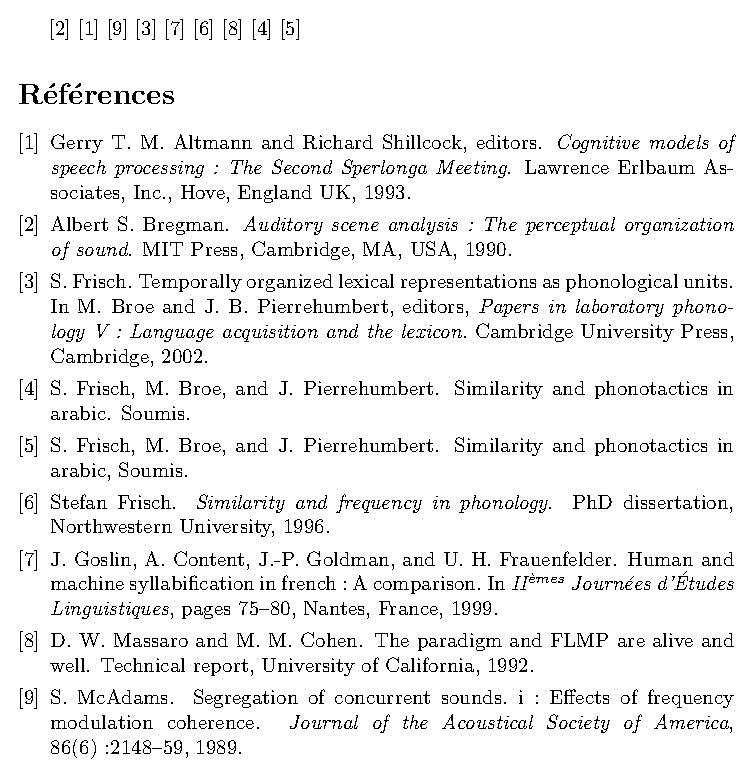
\includegraphics[width=.6\textwidth]{material/plain}
\end{center}

\section{Style \emph{unsrt}}
{\large\verb1\bibliographystyle{unsrt}1}
\begin{center}
  \includegraphics[width=.6\textwidth]{material/unsrt}
\end{center}

\section{Style \emph{abbrv}}
{\large\verb1\bibliographystyle{abbrv}1}
\begin{center}
  \includegraphics[width=.6\textwidth]{material/abbrv}
\end{center}

\section{Style \emph{ieeetr}}
{\large\verb1\bibliographystyle{ieeetr}1}
\begin{center}
  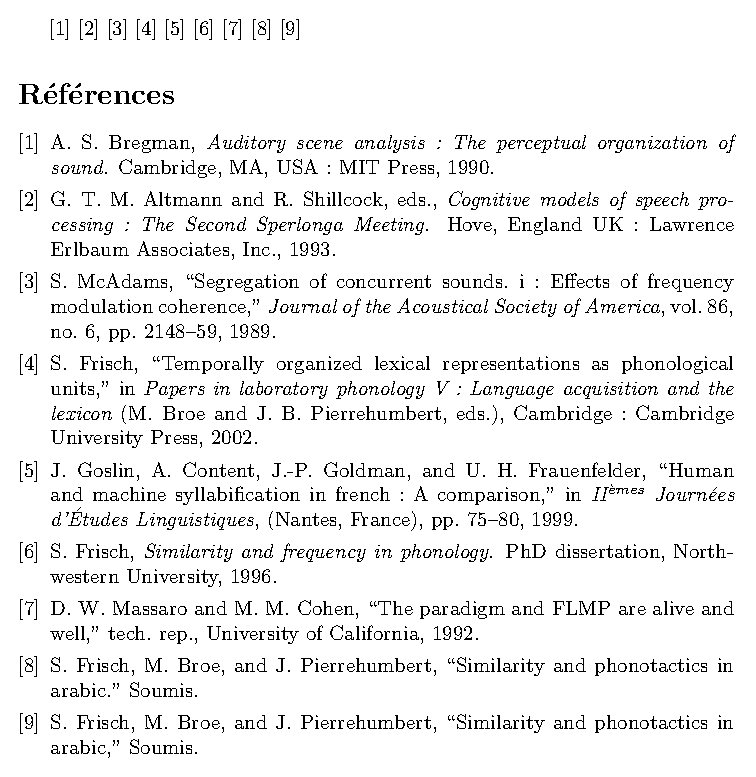
\includegraphics[width=.6\textwidth]{material/ieeetr}
\end{center}

\section{Style \emph{alpha}}
{\large\verb1\bibliographystyle{alpha}1}
\begin{center}
  \includegraphics[width=.6\textwidth]{material/alpha}
\end{center}

\section{Style \emph{siam}}
{\large\verb1\bibliographystyle{siam}1}
\begin{center}
  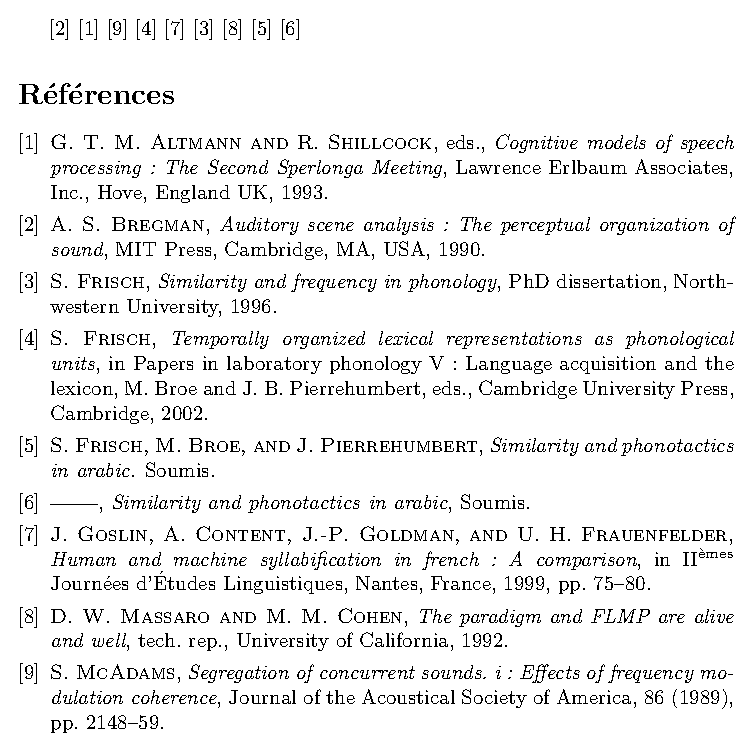
\includegraphics[width=.6\textwidth]{material/siam}
\end{center}

\section{\ldots et en utilisant l'extension \emph{natbib}}
\begin{center}
  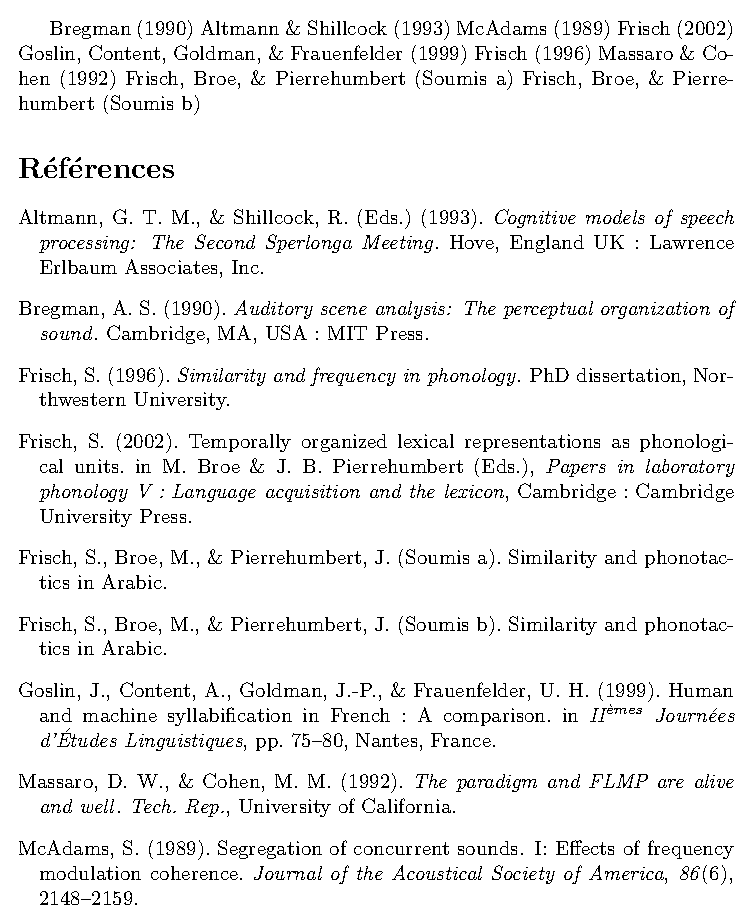
\includegraphics[width=.5\textwidth]{material/natbib-apaformat}
\end{center}





\section{Utilisation de BIB\TeX\  avec \LaTeX}
\pagecolor{\BGColor}
\color{\FGColor}

\vfill
\begin{itemize}
\item Lors de la rédaction du texte, on cite les références bibliographiques en
  désignant l'entrée correspondante dans la base de données bibliographique par
  l'instruction \verb1\cite{clé-de-la-référence}1.
\item La liste des références bibliographiques, sera construite automatiquement
  à la fin du document.
\item On utilise 2 instructions pour contrôler la gestion des références
  bibliographiques :
  \begin{itemize}
  \item \verb1\bibliography{nom-de-fichier}1 indique le nom du fichier contenant
    la base de données bibliographique.
  \item \verb1\bibliographystyle{nom-du-style}1 spécifie l'apparence des appels
    et des références. Les styles \emph{standard} sont :
    \begin{itemize}
    \item plain : [1] Noam Chomsky\ldots
    \item unsrt : idem mais dans l'ordre d'apparition des appels de citation.
    \item abbrv : [1] N. Chomsky\ldots
    \item ieetr : idem mais dans l'ordre d'apparition des appels de citation.
    \item alpha : [Cho68] Noam Chomsky\ldots
    \end{itemize}
  \end{itemize}
\end{itemize}
\vfill




\section{Compilation d'un document}
\label{sec:compilation-bibtex}


\vfill
\begin{itemize}
\item \verb1$ latex1
\item \verb1$ bibtex1
\item \verb1$ latex1
\item \verb1$ latex1
\end{itemize}
\vfill




\section{Exercices}
\label{sec:exercices}
\vfill
\begin{itemize}
\item Créez votre propre base de données bibliographique.
\item Créez un document dans lequel vous allez citer ces références en
  utilisant les techniques précédentes et en choisissant un style
  (plain, alpha, ieeetr\ldots). Nous verrons l'usage de natbib plus
  tard (c'est une extension, pas un style bibliographique).
\item Compilez votre document.
\end{itemize}
\vfill








\chapter{L'extension Ref\TeX\ d'Emacs}
\label{cha:reftex}
\begin{center}
  \begin{minipage}[r]{0.5\linewidth}
    L'extension REF\TeX\ d'Emacs permet de gérer plus facilement le
    processus de citations bibliographiques et de renvois vers les
    parties du document.
  \end{minipage}
\end{center}

\include{inputs/refTeX}


\chapter{Utilisation de l'extension \texttt{natbib}}
\label{cha:natbib}
\begin{center}
  \begin{minipage}[r]{0.5\linewidth}
    L'extension \LaTeX\ \emph{natbib} est une extension
    bibliographique qui permet de produire des bibliographies et des
    appels bibliographiques conformes à certaines exigences n'ayant
    pas été prévues en standard. On retrouve ce type de \og standard
    \fg dans les sciences de la vie mais aussi dans certains
    (sous-)domaines des sciences humaines et sociales (certaines
    branches de la psychologie, de la linguistique, de la sociologie,
    de la géographie\ldots)
  \end{minipage}
\end{center}

\include{inputs/biblio-natbib}


 \chapter{Utilisation de l'extension \texttt{jurabib}}
 \label{cha:jurabib}
 \begin{center}
   \begin{minipage}[r]{0.5\linewidth}
     L'extension \LaTeX\ \emph{natbib} est une extension
     bibliographique qui permet de produire des bibliographies et des
     appels bibliographiques conformes à certaines exigences n'ayant
     pas été prévues en standard. On retrouve ce type de \og standard
     \fg en littérature et dans certains (sous-)domaines des sciences
     humaines et sociales (psychologie, linguistique, philosophie,
     histoire\ldots).

   \end{minipage}
 \end{center}

 \include{inputs/biblio-jurabib}


\chapter{Personnalisation de la mise en page}
\label{cha:personnalisation}
\begin{center}
  \begin{minipage}[r]{0.5\linewidth}
    Ce chapitre vous permettra de mieux comprendre comment on peut
    influencer la mise en page prévue en standard par
    \LaTeX. Modification des formats de page, des marges, des
    paragraphes, des titres de section, en-têtes et pieds de
    page\ldots
  \end{minipage}
\end{center}


\section{Le contrôle des tailles avec \LaTeX}

Dans les pages suivantes, un certain nombre de commandes contrôlent
des dimensions qui prises en compte par \LaTeX\ lors du formatage. Les
dimensions peuvent être exprimées dans différentes unités, parmi
lesquelles :

Les quatre premières unités (cm, mm, in, pt) sont des unités absolues
(leur valeur reste la même quel que soit le contexte dans lequel on se
trouve). Les deux dernières sont des unités dites relatives (leur
valeur réelle dépend du contexte, c'est à dire de la taille de la
police en cours).


\begin{description}
\item[cm] centimètres;
\item[mm] millimètres;
\item[in] pouces (inches);
\item[pt] points (dimension informatique);
\item[ex] taille verticale d'un \emph{x} (permet d'indiquer une taille
  relative à la police utilisée);
\item[em] taille horizontale d'un \emph{m} (permet également
  d'indiquer une taille relative à la police utilisée);
\end{description}

\section{Double interligne}

Dans la plupart des documents universitaires (mais aussi parfois lors
de la soumission d'articles dans des revues scientifiques), il vous
est demandé de fournir des textes avec une interligne double. Il
existe une extension destinée spécifiquement à cet usage :

\begin{verbatim}
\usepackage{setspace}
\doublespacing

ou

\onehalfspacing

\end{verbatim}

Comme d'habitude, l'appel de l'extension se fait dans l'en-tête du
document.

La commande \verb1\doublespacing1 (ou \verb1\onehalfspacing1) est
aussi introduite dans l'en-tête; elle est valable pour l'ensemble du
document.

A priori, vous \emph{ne devez pas} changer ce paramètre en cours de
document. Si toutefois vous tenez absolument à le faire, l'extension
fournit aussi des environnement permettant de changer temporairement
le réglage.


\section{Marges}

L'extension \emph{geometry} permet de contrôler précisément la taille
des marges du document (entre autres). Son utilisation est très simple
:

\begin{verbatim}
\usepackage[left=5cm,right=4cm,bottom=2.5cm,top=2.5cm]{geometry}
\end{verbatim}






\section{Formatage de la page de titre}

Pour formater votre page de titre, vous pouvez, à la place de
l'instruction \verb1\maketitle1 vue au début du cours, utiliser un
code similaire à ce qui suit et l'adapter à votre convenance :


\begin{footnotesize}
\begin{verbatim}
\begin{titlepage}
  \singlespacing
  \sffamily
  \begin{center}
    {\bfseries\large Université de Nantes}\\
    {UFR Lettres et Langages}\\
    {Année Universitaire 2005--2006}\\
    \vfill

    {\Large\bfseries Titre du Mémoire}

    \vspace{2ex} {\large \'Eventuellement un sous-titre}
     
    \vspace{8ex}
    Prénom Nom\\
    Date

    \begin{flushright}
      \vfill
      \begin{tabular}{lr}
        Membres du Jury : & \\
        & Nom, Prénom (directeur du mémoire)\\
        & Nom, prénom\\
      \end{tabular}
    \end{flushright}
    \vspace{8ex}
    
    { Master 2 mention \og Langues et Langages \fg\\
      Spécialité \og Sciences du Langage \fg\\
    Parcours \og Informatisation des Langues \fg\\}
  \end{center}
\end{titlepage}
\end{verbatim}
\end{footnotesize}




\section{En-têtes et Pieds de pages}

Pour contrôler les en-têtes et les pieds de page, on utilise
l'extension \emph{fancyhdr} (pour \emph{fancy headers}). On déclare
que le style de page utilisé sera le style \emph{fancy} (celui produit
par cette extension) et on définit la nature des différentes parties
de ces éléments.

On définit ci-dessous les caractéristiques de l'en-tête droite et
gauche et celles du pied de page au centre (dans lequel on va placer
les numéros de page).

On met ensuite la largeur des lignes de séparation entre l'en-tête et
le texte (et respectivement le pied de page) à 0 points (pas de
lignes).

Les commandes \verb1\rightmark1 et \verb1\leftmark1 permettent de
faire varier le texte de manière automatique (en fonction des classes
de documents, les en-têtes gauche et droit contiendront par exemple
les noms des auteurs, le titre du document, le titre du chapitre en
cours\ldots

\begin{verbatim}
\usepackage{fancyhdr}
\pagestyle{fancy}

\fancyhf{} % ici, on vide les en-têtes et pieds de page avant de les définir

\fancyhead[R]{\small \sffamily En-tête à droite} (on peut par exemple mettre \rightmark)
\fancyhead[L]{\small \sffamily En-tête à gauche} (on peut par exemple mettre \leftmark)
\fancyfoot[C]{\small \sffamily \thepage}
\renewcommand{\headrulewidth}{0pt}
\renewcommand{\footrulewidth}{0pt}
\end{verbatim}


\section{Personnalisation des titres de section (mode de numérotation)}

On contrôle le mode de numérotation en redéfinissant les commandes
suivantes (qui sont utilisées automatiquement par \LaTeX\ lors de la
compilation). Il convient, au préalable, de \emph{relever} la
profondeur de section au-delà de laquelle s'interrompt la numérotation
des sections.

{\small
\begin{verbatim}
\setcounter{secnumdepth}{7}

\def\thechapter{\Roman{chapter}}
\def\thesection{\Alph{section}}
\def\thesubsection{\Roman{subsection}}
\def\thesubsubsection{\arabic{subsubsection}}
\def\theparagraph{\roman{paragraph}}
\def\thesubparagraph{\alph{subparagraph}}
\end{verbatim}
}

\section{Personnalisation des titres de section (changement de mise en forme simple)}

On fait appel à l'extension \emph{sectsty} et on redéfinit chaque
niveau de section (alignement du texte, taille de la police, graisse,
type de police, éventuellement suppression de la numérotation des
pages, insertion d'un saut de page préalable).

{\small
\begin{verbatim}
\usepackage{sectsty}

%\partfont{\centering\Huge\bfseries\sffamily\thispagestyle{empty}}
%\chapterfont{\Large\bfseries\sffamily}
\sectionfont{\newpage\raggedleft\large\bfseries\sffamily}
\subsectionfont{\large\mdseries\sffamily}
\subsubsectionfont{\normalsize\mdseries\sffamily}
\end{verbatim}
}


\section{Personnalisation des titres de section (changement de mise en forme plus complexe)}

On fait appel à l'extension \emph{titlesec} (et ici on ajoute un
recours à l'extension \emph{scalefont} qui permet de gérer plus
finement les tailles de police). Le format des commandes est le suivant :

{\small
\begin{verbatim}
\titleformat{niveau}[formatage du paragraph]{formatage du titre}{formatage du numéro}...
                          ...{espacement entre numéro et titre}{code à insérer après le titre}
\end{verbatim}
}

{\scriptsize
\begin{verbatim}
\usepackage{scalefnt}
\usepackage{titlesec}

\titleformat{\part}[display]{\raggedleft\Huge\scalefont{1.3}\sffamily\bfseries\thispagestyle{empty}}{\partname}{0cm}{}
\titleformat{\chapter}[display]{\raggedleft\Huge\sffamily\bfseries}{\chaptertitlename\ \thechapter}{0cm}{}
\titleformat{\section}{\Large\sffamily\bfseries}{\thesection)\quad}{0cm}{}
\titleformat{\subsection}{\Large\sffamily}{\thesubsection --\quad}{0cm}{}
\titleformat{\subsubsection}{\large\sffamily\itshape\raggedright}{\thesubsubsection.\quad}{0cm}{}
\titleformat{\paragraph}{\normalsize\sffamily\itshape\raggedright}{\theparagraph\quad}{0cm}{}
\titleformat{\subparagraph}{\normalsize\sffamily\itshape\raggedright}{\thesubparagraph\quad}{0cm}{}
\end{verbatim}
}


\section{Modification des paragraphes}

On peut modifier très simplement l'indentation par défaut (espace en
début de ligne lors des changements de paragraphe) et l'espacement
vertical entre paragraphes :

\begin{verbatim}
\setlength{\parindent}{0cm}
\setlength{\parskip}{1em}
\end{verbatim}



\section{Et maintenant ?}

Si vous avez réussi à tenir jusqu'au bout, alors vous êtes sur la
bonne voie\ldots mais votre apprentissage est loin d'être fini. Il
existe très certainement un millier de choses que vous souhaiteriez
pouvoir faire sans encore savoir comment vous pourriez vous y prendre
avec \LaTeX. Il vous faudra faire preuve de beaucoup de patience et
d'un travail régulier, lire la documentation qui fourmille sur
internet, vous procurer un livre (éventuellement en format
électronique, cf. les références données p.~\pageref{sec:freebooks}),
rechercher des extensions qui pourraient répondre à vos besoins en
consultant le \emph{Comprehensive Tex Archive Network}
(p.~\pageref{sec:websites}).

N'hésitez pas aussi à rechercher la réponse à vos problèmes dans les
foires aux question (p.~\pageref{sec:faq}) et à consulter
régulièrement les \emph{newsgroups} (p.~\pageref{sec:newsgroups}).

\vfill

\hfill Bon courage\ldots et bonne route avec \LaTeX !

\vfill


% double interligne
% geometry
% formatage page de titre (standard Université)
              




% \chapter{L'indexation des documents}
% \include{indexation-LaTeX}


% \chapter{Recherche et Installation d'extensions supplémentaires}
% \include{inputs/install-LaTeX-extensions}


% \chapter{Questions et problèmes divers}
% \include{inputs/misc-LaTeX}


% \chapter{Outils pour la linguistique}
% \include{inputs/linguistique.tex}


\listoffigures
\label{list:fig}

\listoftables
\label{list:tab}

%\listof{exemple}{Liste des exemples}

%\newpage
% \vspace*{4cm}
% \begin{center}
% \large Ce document peut-être téléchargé sur le site :\\
% \url{http://www.lettres.univ-nantes.fr/sdl/teaching/master/latex/}  
% \end{center}
% \vfill


%%% Local Variables: 
%%% mode: latex
%%% TeX-master: "ED-Initiation-LaTeX-couleur"
%%% End: 

